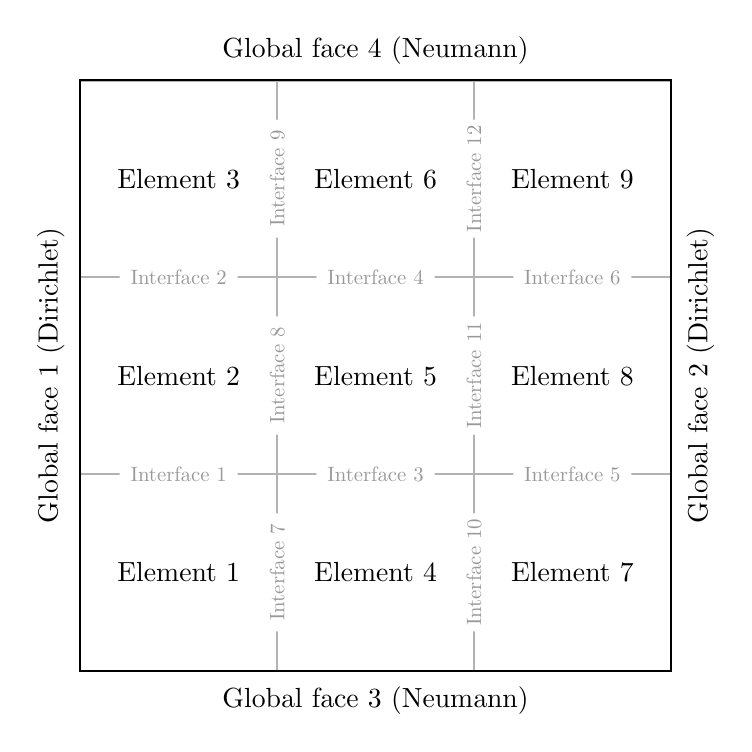
\begin{tikzpicture}[scale=2.5]
\draw[step=1cm,black!30,line width=0.3mm] (0, 0) grid (3, 3);
\draw[line width=0.3mm] (0, 0) rectangle (3, 3);

\fill[white] (0.5cm, 1cm) circle (0.3cm);
\node[color=black!40, scale=0.75] at (0.5cm, 1cm) {Interface 1};
\fill[white] (0.5cm, 2cm) circle (0.3cm);
\node[color=black!40, scale=0.75] at (0.5cm, 2cm) {Interface 2};
\fill[white] (1.5cm, 1cm) circle (0.3cm);
\node[color=black!40, scale=0.75] at (1.5cm, 1cm) {Interface 3};
\fill[white] (1.5cm, 2cm) circle (0.3cm);
\node[color=black!40, scale=0.75] at (1.5cm, 2cm) {Interface 4};
\fill[white] (2.5cm, 1cm) circle (0.3cm);
\node[color=black!40, scale=0.75] at (2.5cm, 1cm) {Interface 5};
\fill[white] (2.5cm, 2cm) circle (0.3cm);
\node[color=black!40, scale=0.75] at (2.5cm, 2cm) {Interface 6};

\fill[white](1cm, 0.5cm) circle (0.3cm);
\node[color=black!40, rotate=90, scale=0.75] at (1cm, 0.5cm) {Interface 7};
\fill[white] (1cm, 1.5cm) circle (0.3cm);
\node[color=black!40, rotate=90, scale=0.75] at (1cm, 1.5cm) {Interface 8};
\fill[white] (1cm, 2.5cm) circle (0.3cm);
\node[color=black!40, rotate=90, scale=0.75] at (1cm, 2.5cm) {Interface 9};
\fill[white] (2cm, 0.5cm) circle (0.3cm);
\node[color=black!40, rotate=90, scale=0.75] at (2cm, 0.5cm) {Interface 10};
\fill[white] (2cm, 1.5cm) circle (0.3cm);
\node[color=black!40, rotate=90, scale=0.75] at(2cm, 1.5cm) {Interface 11};
\fill[white] (2cm, 2.5cm) circle (0.3cm);
\node[color=black!40, rotate=90, scale=0.75] at (2cm, 2.5cm) {Interface 12};


\draw (0.5cm, 0.5cm) -- (0.5cm, 0.5cm) node[anchor=center] {Element 1};
\draw (0.5cm, 1.5cm) -- (0.5cm, 1.5cm) node[anchor=center] {Element 2};
\draw (0.5cm, 2.5cm) -- (0.5cm, 2.5cm) node[anchor=center] {Element 3};
\draw (1.5cm, 0.5cm) -- (1.5cm, 0.5cm) node[anchor=center] {Element 4};
\draw (1.5cm, 1.5cm) -- (1.5cm, 1.5cm) node[anchor=center] {Element 5};
\draw (1.5cm, 2.5cm) -- (1.5cm, 2.5cm) node[anchor=center] {Element 6};
\draw (2.5cm, 0.5cm) -- (2.5cm, 0.5cm) node[anchor=center] {Element 7};
\draw (2.5cm, 1.5cm) -- (2.5cm, 1.5cm) node[anchor=center] {Element 8};
\draw (2.5cm, 2.5cm) -- (2.5cm, 2.5cm) node[anchor=center] {Element 9};


\node[rotate=90] at (-0.15cm, 1.5cm) {Global face 1 (Dirichlet)};
\node[rotate=90] at (3.15cm, 1.5cm) {Global face 2 (Dirichlet)};
\node at (1.5cm, -0.15cm) {Global face 3 (Neumann)};
\node at (1.5cm, 3.15cm)  {Global face 4 (Neumann)};
\end{tikzpicture}